\documentclass[UserManual.tex]{subfiles}
\begin{document}
\setcounter{section}{1}

\section{Installation and Getting Started}\label{sec:installation}

\subsection{Prerequisites}
{\it Smooth Emulator} software should run on UNIX, Mac OS or Linux, but is not supported for Windows OS. {\it Smooth Emulator} is largely  written in C++. In addition to a C++ compiler (CMake files assume you have C++ 20 standard), the user needs the following software installed.

\begin{itemize}
    \item git
    \item CMake
    \item Eigen3 (Linear Algebra Package)
    \item Python/Matplotlib (only for generating plots in the MCMC procedure)
\end{itemize}

CMake is an open-source, cross-platform build system that helps automate the process of compiling and linking for software projects. Hopefully, CMake will perform the needed gymnastics to find the Eigen3 installation. To install CMake, either visit the CMake website (https://cmake.org/), or use the system's package manager for the specific system. For example, on Mac OS, if one uses {\it homebrew} as a package manager, the command is
{\tt 
\begin{verbatim} % brew install cmake\end{verbatim}
}

Eigen is a C++ template library for vector and matrix math, i.e. linear algebra. The user can visit the Eigen website (\url{https://eigen.tuxfamily.org/dox/}), or use their system's package manager. For example on Mac OS with {\it homebrew},
{\tt 
\begin{verbatim} % brew install eigen\end{verbatim}
}

\subsection{Downloading the Repository}

The software requires downloading the BAND framework software repository into some directory. Should that be in the User's home directory, the User might enter
{\tt 
\begin{verbatim}
    /Users/CarlosSmith% git clone https://github.com/bandframework/bandframework.git
\end{verbatim}
}
Within the repository, there will be a directory\\{\tt /Users/CarlosSmith/bandframework/software/SmoothEmulator/}. All the relevant functionality of {\it Smooth Emulator} is contained within this directory. Throughout the manual the phrase {\tt \$\{GITHOME\_BAND\_SMOOTH\}} will refer to this directory. 

The User needs to create a personal directory from which the User would perform most projects. This is easiest accomplished by copying a template from the {\it Smooth} distribution. For example
{\tt
\begin{verbatim}
    % cp -r ${GITHOME_BAND_SMOOTH}/templates /Users/CarlosSmith/mysmoothy
\end{verbatim}
}
Within this directory one will find a template project directory, which for the template would then be {\tt /Users/CarlosSmith/mysmoothy/myproject}. 
Hence forth, {\tt \$\{MY\_PROJECT\}} is a name chosen by the User, and will refer to this directory, including the path, from which the User will perform most of the analysis. The User may wish to have several such directories, located according to the User's preference. Any time a new analysis is performed with new parameters, and if the User wishes to save the previous analysis, a new {\tt \$\{MY\_PROJECT\}} directory should be created. These directories should be outside the main distribution, i.e. outside the {\tt bandframework/} path so that the User's work does not interfere with the repository. 

Within the {\tt templates/} directory, there is also a directory {\tt ../templates/mylocal/}, which after the copying above will become: {\tt /Users/CarlosSmith/mysmoothy/mylocal}. The {\tt mylocal/} directory contains the main programs and the {\it Smooth Emulator} executables which will be stored in {\tt \$\{GITHOME\_BAND\_SMOOTH\}/mylocal/bin}. Because the User might wish to edit the main programs, or to add similar programs, this provides the User a space to make such edits, all while leaving an original copy of the directory in the {\tt templates/} directory. 

For the remainder of this manual, {\tt \$\{GITHOME\_BAND\_SMOOTH\}}, {\tt \$\{MY\_LOCAL\}} and {\tt \$\{MY\_PROJECT\}} will be used to denote the location of these directories.

\subsection{Directory and File Structure}

\begin{figure}
\centerline{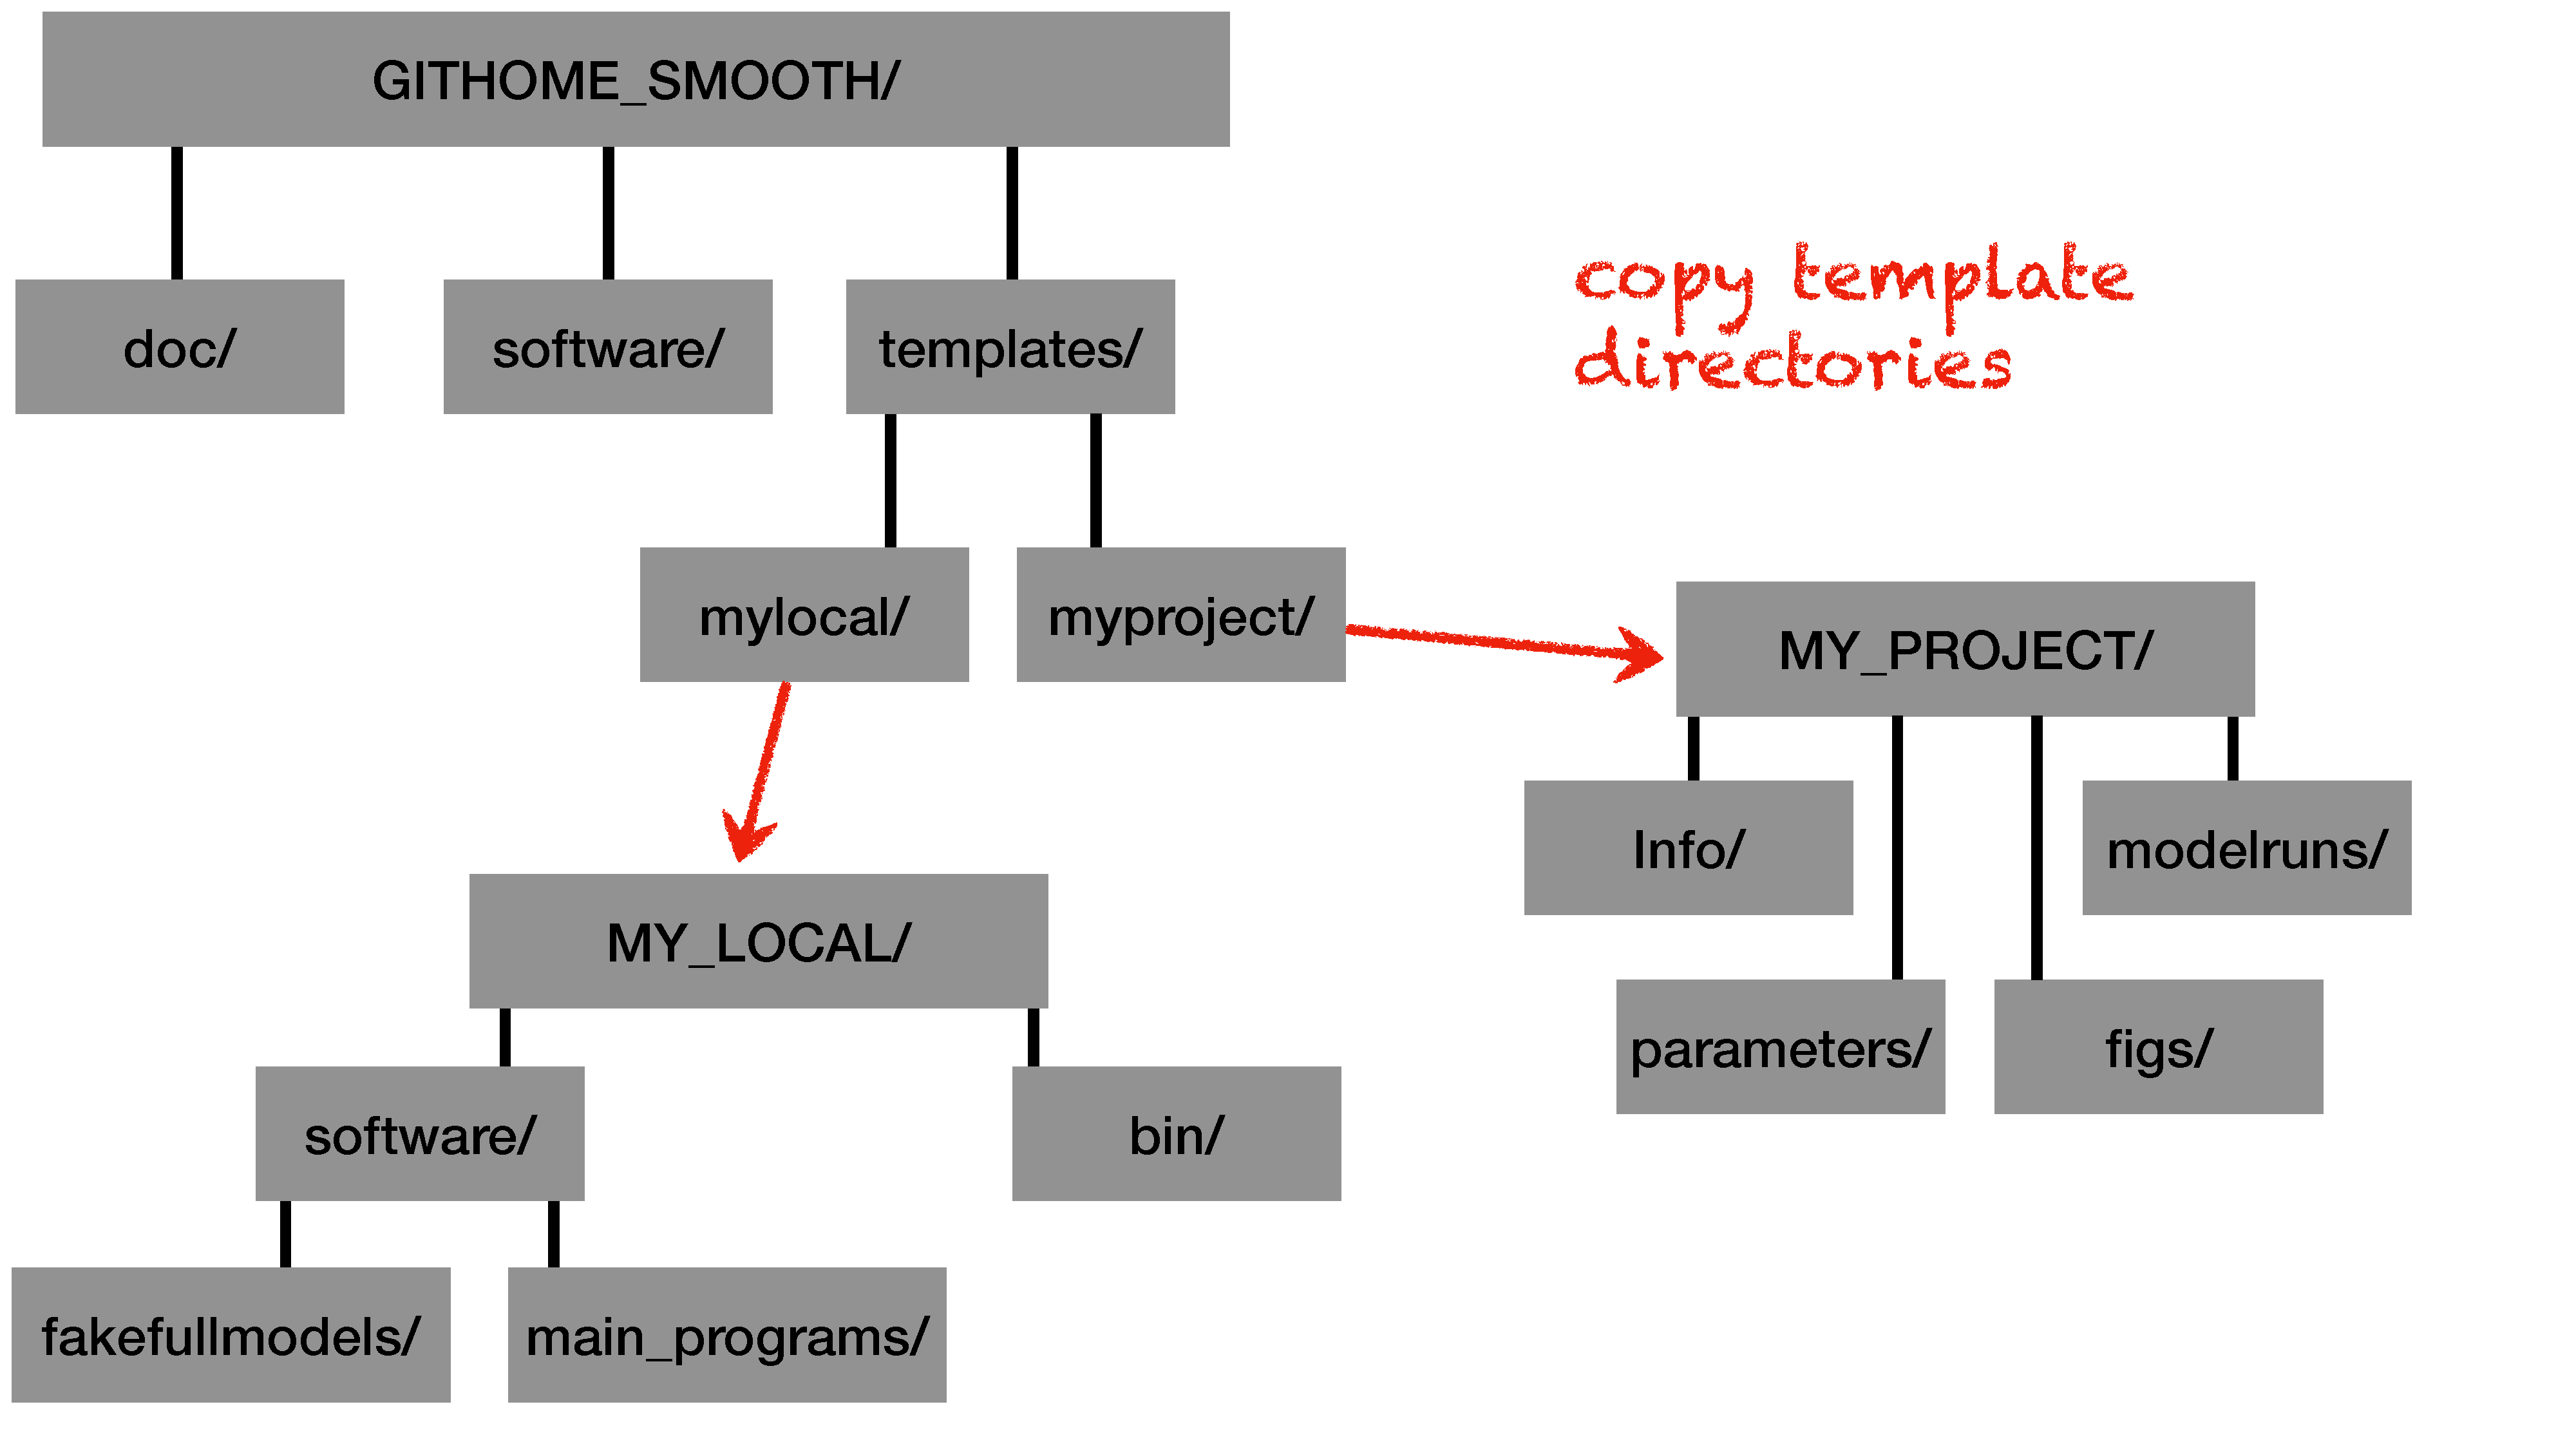
\includegraphics[width = 0.85\textwidth]{figs/directorystructure}}
\caption{{\bf The directory structure}: The User clones the repository into some location, which will be referred to as {\tt \$\{\tt GITHOME\_BAND\_SMOOTH\}}. The User can then copy the {\tt  \$\{MY\_PROJECT\}} directory to the User's choices of locations outside the path of the BAND repository.  The programs are designed to be run from within the {\tt \$\{MY\_PROJECT\}/} directory, which also where data files related to the project will be located. The User can make multiple copies of {\tt  \$\{MY\_PROJECT\}} whenever they wish to run and save different instances of {\it Smooth Emulator}. All {\it Smooth Emulator} executables are designed to be run from the {\tt \$\{MY\_PROJECT\}/} directory. Within that directory there is a subdirctory, {\tt  \$\{MY\_PROJECT\}/smooth\_data/}, within which the data files used by {\it Smooth Emulator} reside. The actual executables will be stored in the {\tt  \$\{MY\_LOCAL\}/bin} directory. The main programs are also located in this path, while the libraries will be located in the main repository path. This design was made with the idea that the User might wish to create their own versions of the main programs, and store them outside the repository structure.
}
\end{figure}

The {\tt \$\{GITHOME\_BAND\_SMOOTH\}/software/} directory contains codes that are used to create libraries specific to the sampler and emulator. The User can change to The executables are stored in {\tt \$\{MY\_LOCAL\}/bin}. The short main program source files are located in\\{\tt \$\{MY\_LOCAL\}/software/main\_programs}. It is not envisioned that the User would edit files in the\\{\tt SmoothEmulator/software/} directory, but that the User may well wish to create custom versions of the short main programs in {\tt \$\{MY\_LOCAL\}/software/main\_programs/}. The main programs are compiled using the CMake files in {\tt \$\{MY\_LOCAL\}/software/main\_programs/}. The User may find it convenient to add {\tt \$\{MY\_LOCAL\}/bin/} to their path.

\subsection{Compiling Libraries }

First, change into software directories, then create the makefiles with cmake, then compile them.
{\tt 
\begin{verbatim}
    % cd ${GITHOME_BAND_SMOOTH}/software
    ${GITHOME_BAND_SMOOTH}/software% cmake .
    ${GITHOME_BAND_SMOOTH}/software% make
\end{verbatim}
}
There seems to be a common problem that {\tt cmake} misreports the path of the {\tt Eigen} installation. If the User should get an error stating that the Eigen header files cannot be found, the User can set the environmental variable,
{\tt 
\begin{verbatim}
    % export EIGEN3_INCLUDE_DIR=/usr/local/include/eigen3
\end{verbatim}
}
The final arguments may need to be changed depending on the User's location of the packages. If the User wishes to choose a specific C++ compiler, the {\tt cmake} command should be replaced with {\tt cmake -D CMAKE\_CXX\_COMPILER=g++-11}, or whichever compiler is preferred. 

At this point all the libraries are built, but this does not include the main programs. The main programs are short, and are meant to serve as examples which the User might copy and edit at will. Before compiling, one needs to set an environmental variable so that the compilation can find the libraries needed for compilation.
{\tt
\begin{verbatim}
  % export GITHOME_BAND_SMOOTH=/Users/CarlosSmith/bandframework/software/SmoothEmulator
\end{verbatim}
}
The first part of the path needs to be replaced with the location of the {\tt bandframework} git repository. If one prefers not to set an environmental variable, one can instead edit\\
{\tt \$\{MY\_LOCAL\}/software/CMakeLists.txt}, and replace the line where the variable {\tt GITHOME\_BAND\_SMOOTH} is set to the shell's environmental variable with one where it is set explicitly.

Below, this illustrates how to compile the programs used for generating training points with Simplex and for tuning the emulator with {\it Smooth Emulator}:
{\tt
\begin{verbatim}
    % cd ${MY_LOCAL}/software
    ${MY_LOCAL}/software% cmake .
    ${MY_LOCAL}/software% make
    .
    .
\end{verbatim}
}
The {\tt cmake} command will also recompile the main libraries in {\tt \$\{GITHOME\_BAND\_SMOOTH\}/software/} if necessary. Several source codes for main programs can be found in\\
{\tt \$\{MY\_LOCAL\}/software/main\_programs/}. If you build your own main programs (probably using these as examples), you can edit the {\tt CMakeList.txt} file in {\tt \$\{MY\_LOCAL\}/software/main\_programs/}, using the existing entries as an example. The executables should appear in {\tt \$\{MY\_LOCAL\}/bin/}. 

\subsection{The {\tt MY\_PROJECT} Directory}

Within {\tt \$\{MY\_PROJECT\}/smooth\_data} there are several sub-directories (assuming it was created from the template). The first is {\tt smooth\_data/Info/}. Information about the model parameters, and their priors is stored in {\tt smooth\_data/Info/modelpar\_info.txt}, and information about the observables is stored in {\tt smooth\_data/Info/observable\_info.txt}. The file {\tt smooth\_data/Info/experimental\_info.txt} stores information about the measurements for each observable, and is not needed for building the emulator, but is used by the MCMC investigation of the posterior.

The {\tt smooth\_data/smooth\_parameters} directory stores user-defined parameter files used by {\it Simplex Sampler}, {\tt smooth\_data/smooth\_parameters/simplex\_parameters.txt}, and by {\it Smooth Emulator}\\{\tt smooth\_data/smooth\_parameters/emulator\_parameters.txt}. These are user-defined parameters related to choices in running the emulation programs, not model parameters.

The directories {\tt smooth\_data/modelruns/run0/}, {\tt  .../modelruns/run1}, $\cdots$, have files describing the model parameters for each run, along with the output required by the emulator for each specific full-model run. For example, the {\tt  smooth\_data/modelruns/run1/} directory has the files {\tt mod\_parameters.txt} and {\tt obs.txt}. The first file stores the model parameter values for that particular training run. The User then runs their full model based on those parameters and stores the corresponding observables in {\tt obs.txt}. The User may generate the {\tt mod\_parameters.txt} files using {\it Simplex Sampler}, or the user might generate them according to some other prescription. Once the User has then generated the {\tt obs.txt} files, {\it Smooth Emulator} can then build and tune the emulator.

Finally the {\tt\$\{MY\_PROJECT\}/figs} directory contains python scripts for plotting results.

\end{document}
